\documentclass[9pt]{pnas-new}
% Use the lineno option to display guide line numbers if required.
% Note that the use of elements such as single-column equations
% may affect the guide line number alignment. 

%\RequirePackage[english,slovene]{babel} % when writing in slovene
\RequirePackage[slovene,english]{babel} % when writing in english
\DeclareUnicodeCharacter{202F}{ }
\templatetype{pnasresearcharticle} % Choose template 
% {pnasresearcharticle} = Template for a two-column research article
% {pnasmathematics} = Template for a one-column mathematics article
% {pnasinvited} = Template for a PNAS invited submission

\selectlanguage{english}
%\etal{in sod.} % comment out when writing in english
%\renewcommand{\Authands}{ in } % comment out when writing in english
%\renewcommand{\Authand}{ in } % comment out when writing in english

\newcommand{\set}[1]{\ensuremath{\mathbf{#1}}}
\renewcommand{\vec}[1]{\ensuremath{\mathbf{#1}}}
\newcommand{\uvec}[1]{\ensuremath{\hat{\vec{#1}}}}
\newcommand{\const}[1]{{\ensuremath{\kappa_\mathrm{#1}}}} 

\newcommand{\num}[1]{#1}

\graphicspath{{./fig/}}

\title{Simulation of group behaviour during a protest}

% Use letters for affiliations, numbers to show equal authorship (if applicable) and to indicate the corresponding author
\author{Nik Čadež}
\author{Pedro Nuno Ferreira Moura de Macedo}
\author{Primož Mihelak}
\author{Luka Bajić}

\affil{Collective behaviour course research seminar report} 

% Please give the surname of the lead author for the running footer
\leadauthor{Čadež} 

\selectlanguage{english}

% Please add here a significance statement to explain the relevance of your work
\significancestatement{By conducting simulations of protests using various models for different subgroups of people, we hope to gain some insight into group behaviour during such events, that might make them logistically easier to organize/control in the future.}{Simulation | group behaviour | crowd control}

\selectlanguage{english}

% Please include corresponding author, author contribution and author declaration information
%\authorcontributions{Please provide details of author contributions here.}
%\authordeclaration{Please declare any conflict of interest here.}
%\equalauthors{\textsuperscript{1}A.O.(Author One) and A.T. (Author Two) contributed equally to this work (remove if not applicable).}
%\correspondingauthor{\textsuperscript{2}To whom correspondence should be addressed. E-mail: author.two\@email.com}

% Keywords are not mandatory, but authors are strongly encouraged to provide them. If provided, please include two to five keywords, separated by the pipe symbol, e.g:
\keywords{Simulation | group behaviour | crowd control} 

\begin{abstract}
The purpose of our project is to study the behavior of a crowd during a protest. In order to so, we will first create a unified modular development environment that implements the basic flocking model. Then we will add obstacle avoidance and place the model in a topological map of Ljubljana. Furthermore, we will divide agents into different groups (e.g. leader, regular protest member and bystander) and create different behavioural patterns for each group based on human psychology. Finally, we will add agents for crowd control (e.g. police) and examine the effect they have on the behaviour of the crowd. Optional: we will attempt to optimize police behaviour with methods such as genetic algorithms (the purpose being crowd dispersal or redirection).
\end{abstract}

\dates{\textbf{\today}}
\program{BMA-RI}
\vol{2024/25}
\no{Group A} % group ID
%\fraca{FRIteza/201516.130}

\begin{document}

% Optional adjustment to line up main text (after abstract) of first page with line numbers, when using both lineno and twocolumn options.
% You should only change this length when you've finalised the article contents.
\verticaladjustment{-2pt}

\maketitle
\thispagestyle{firststyle}
\ifthenelse{\boolean{shortarticle}}{\ifthenelse{\boolean{singlecolumn}}{\abscontentformatted}{\abscontent}}{}

% If your first paragraph (i.e. with the \dropcap) contains a list environment (quote, quotation, theorem, definition, enumerate, itemize...), the line after the list may have some extra indentation. If this is the case, add \parshape=0 to the end of the list environment.
\dropcap{P}rotests are a widespread phenomenon involving typically large groups of people, oftentimes with different, or even conflicting goals between their respective subgroups. As such they are a fascinating subject for studies in various fields, from human psychology to group behaviour simulations, which will be our primary focus during the course of this project. 

\bigskip
The central idea for the project was inspired specifically by the 2020 protests in Ljubljana, that had a distinguishing feature of having an individual leader, but we will try to make our model applicable more generally (for instance, with minor parameter adjustments, we should be able to easily model sports riots or other similar events with various subgroups).  



\section*{Related work}

There are many existing attempts to model protest behaviour, but our project will primarily build on concepts proposed in \cite{protests}. The basic idea is to split the agents into subgroups depending on their level of involvement with the protest. The proposed subgroups are:
\begin{itemize}
    \item active protesters (which are further divided by their level of "passion" or "interest" in the protest), 
    \item bystanders (which may or may not at one point be persuaded to become active protesters, based on parameters discussed in \cite{sportsriots}),
    \item media (which we will likely ignore, as it will not be relevant to our observations): agents attracted to moving in the direction (in their field of view) where the most significant "action" is taking place,
    \item police/crowd control agents (described in more detail in \cite{crowdcontrol2}): their primary goal is dispersing a crowd or redirecting it in a specific direction.
\end{itemize}

\bigskip
Note: if we are intending to model specifically the 2020 Ljubljana protests, we need to additionally implement the concept of a leader, who is to a large extent controlling the movement of all active protesters within a given range, but as such also becomes a more significant target for crowd control agents. 

\bigskip
We will attempt to model behaviour of each of the aforementioned subgroups by assigning them a parameter vector based on human psychology. These parameters are intended to cover a wide range of human emotion, such as willingness to participate in a protest (to determine how likely it is that a bystander will join a protest if the majority of agents in their vicinity are active protesters), inclination towards violence, etc. In \cite{sportsriots} these parameters are referred to as levels of recruitment and defection (willingness) and "mild unrest", "moderate unrest" and "severe unrest" (levels of violence). 


\bigskip
For crowd control agents, we will primarily be using ideas presented in \cite{crowdcontrol2}. The goal is to experiment with different formations of these agents to achieve maximum success rate in terms of crowd dispersal. The effectiveness of these agents should also vary depending on parameters attributed to an individual protester agent. Effectively this means there should be different levels of cooperation with the police depending on which subgroup a protester belongs to. Depending on the level of detail we are aiming for, we might also differentiate between different subgroups of police agents (e.g. more intimidating/less intimidating). 

\section*{Methods}

Implementation of the model will be done in Unity, in a 2-dimensional space observed from bird's-eye view. First step will be the creation of a topological map of Ljubljana. For the time being we have chosen an area of ......$m^2$, but we might expand if necessary. To ensure the correct scale and proportions, we used Google Maps for this step and we took into account the estimated maximum numbers of people that can fit into spaces of particular dimensions. In other words, we attempted to create an environment that's as realistic as possible, so that the obtained results will potentially be useful in various practical applications. 

\bigskip
We plan to perform experiments on various initial group sizes (as mentioned, agents can at some point deflect to another group depending on "willingness" parameter), but for the time being we have chosen the following amounts of agents per group:
\begin{itemize}
    \item active protesters: 250
    \item bystanders: 200
    \item police: 50
    \item leader: 1
\end{itemize}

One of the experiments will be to determine the smallest police to protester ratio for which the crowd control is still effective (i.e. a crowd is successfully dispersed). 

\bigskip
Finally, we will attempt to optimize police behaviour (i.e. find different formations) using approaches such as genetic algorithms to observe if we can further decrease the number of necessary crowd control agents, while maintaining the same effectiveness in terms of crowd dispersal. 

\section*{Results}

So far we have implemented a simulation that incorporates four groups of agents in the same scene and we have defined different movement and interaction parameters for each of them. 

\begin{figure}[H]
\begin{center}
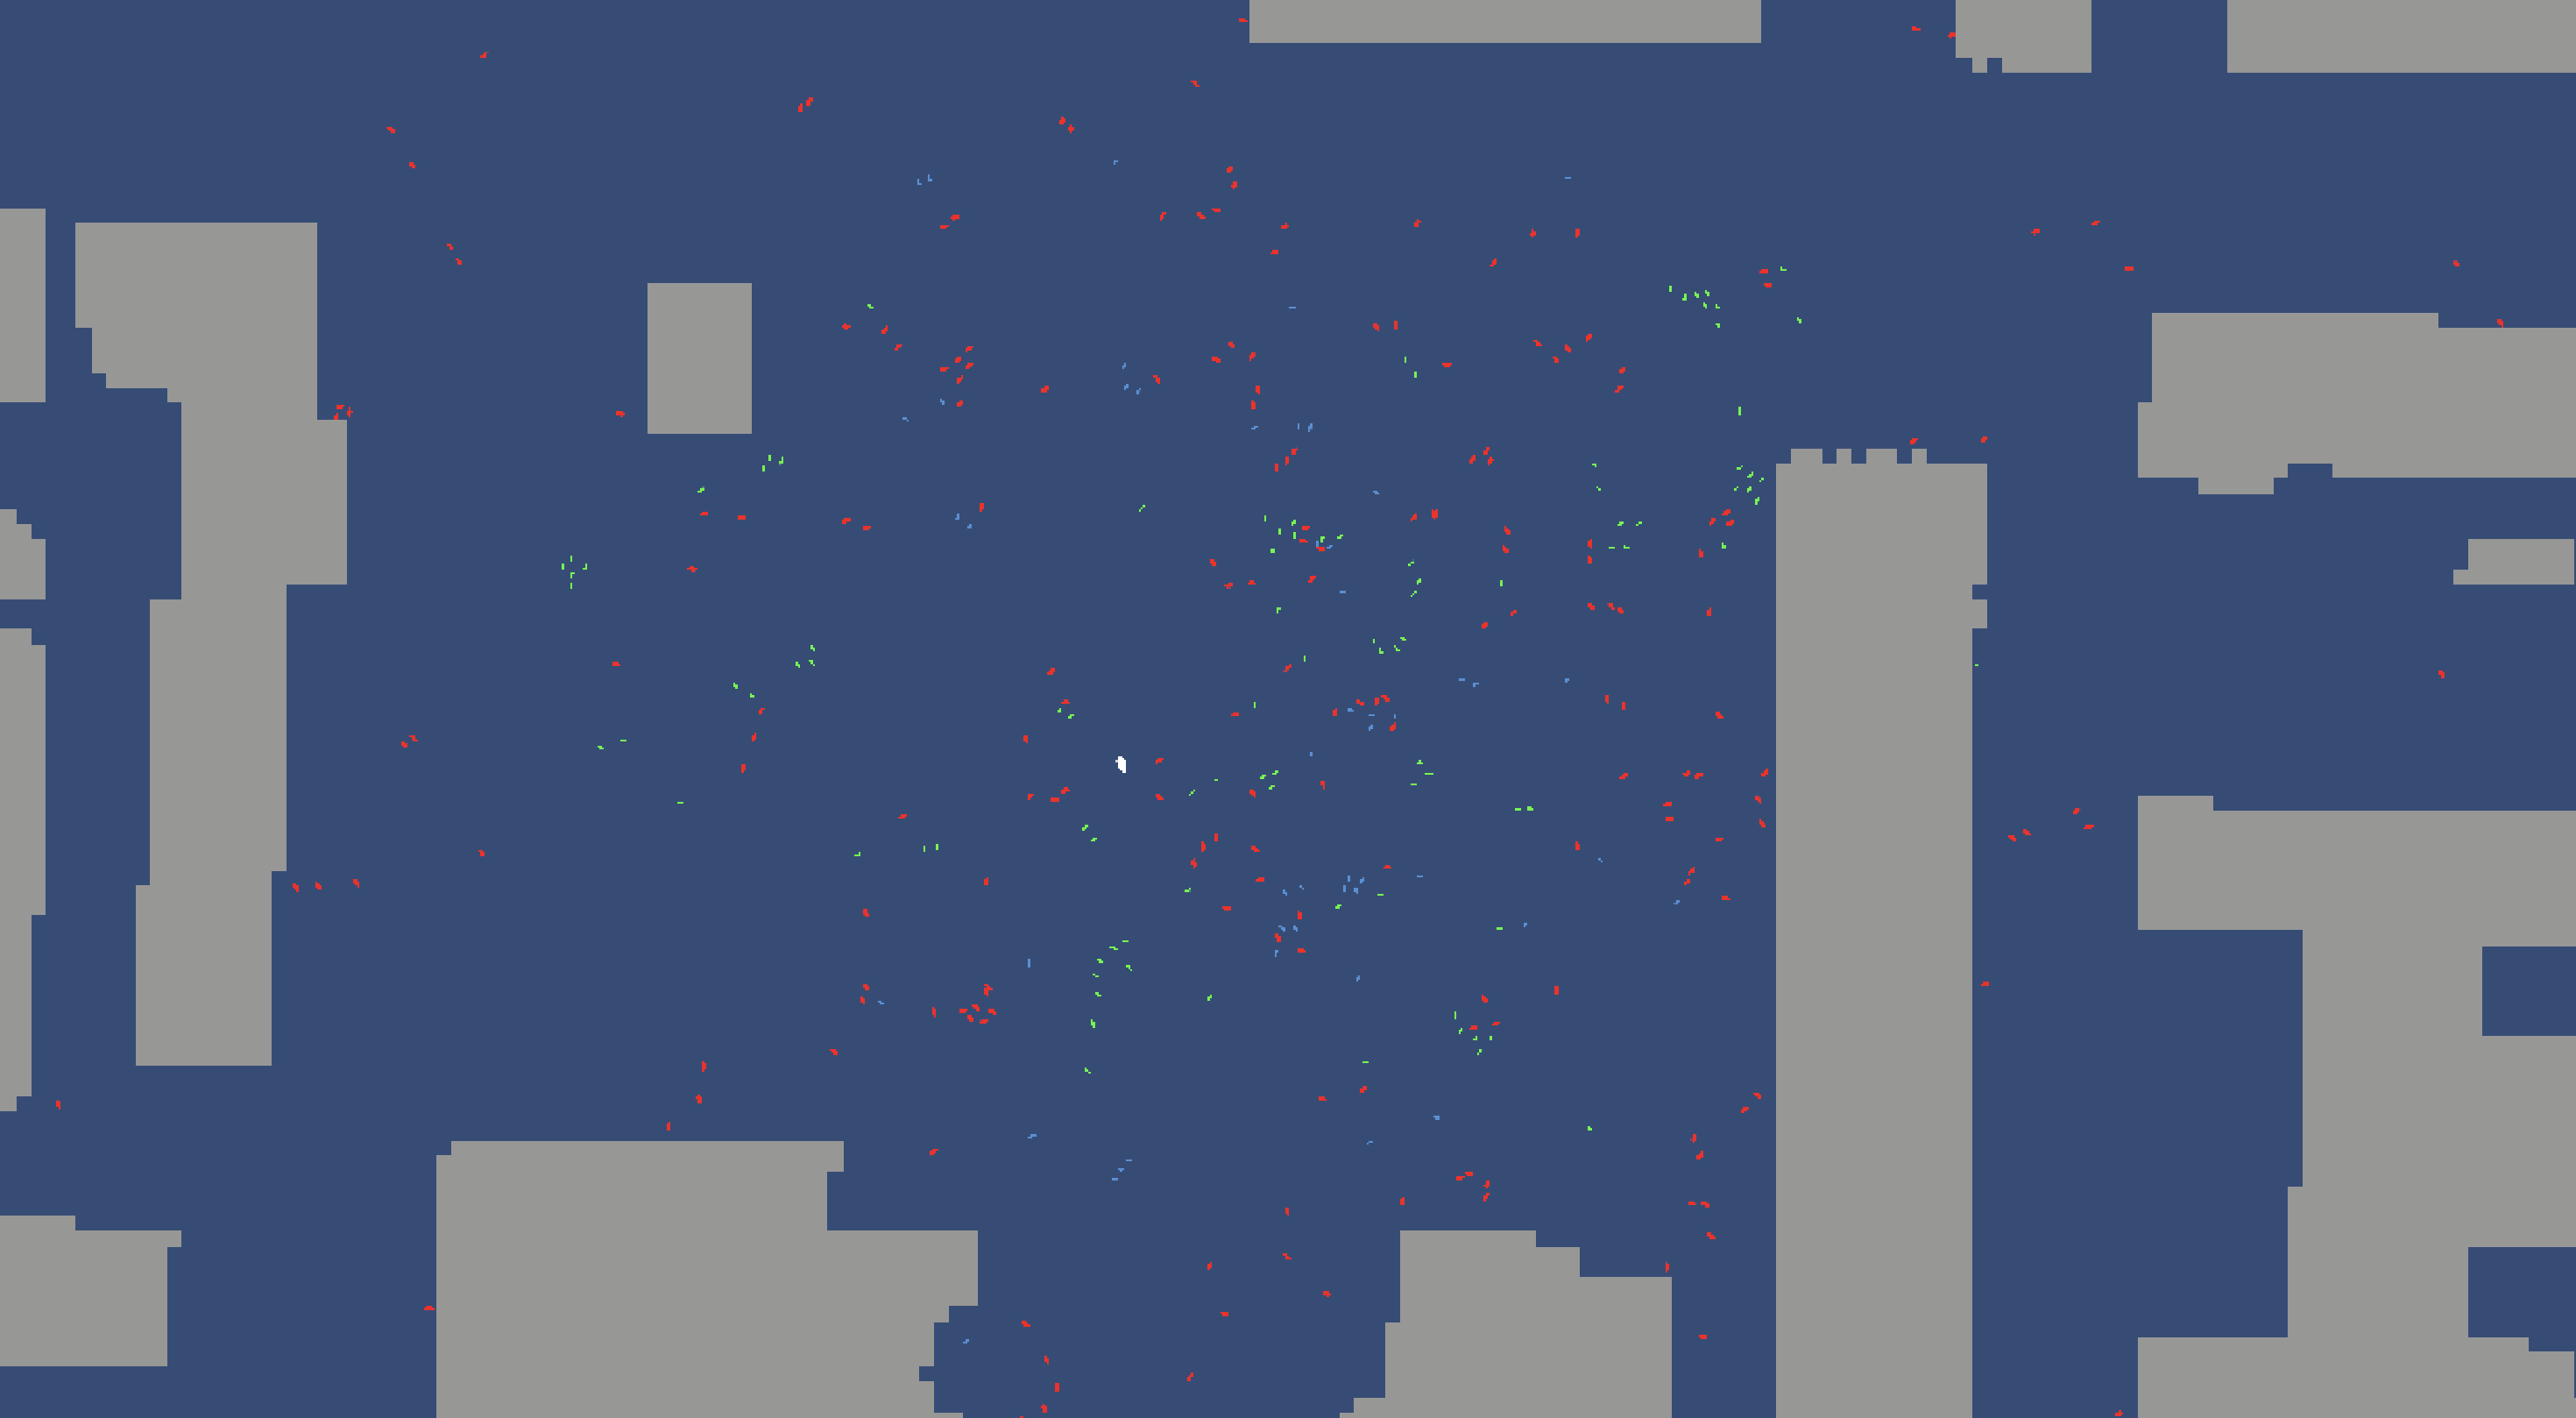
\includegraphics[width=0.8\columnwidth]{simulation.png}
\end{center}
\caption{Example of a protest visualization in Unity: three groups of agents (protesters, bystanders, police) and a topological map of buildings}
\label{fig1}
\end{figure}


\section*{Discussion}

The project is currently progressing according to plan. The implemented model is scalable and modifiable, so we expect to mostly focus on parameter optimization for the remainder of the project. Current challenges are mostly related to effectively and realistically incorporating human psychology into the model. 


\acknow{NČ implemented agent movement and interaction between different groups, PNM worked on the map, PM optimized parameters and improved the visualization, LB did image processing for the map, implemented the baseline model and wrote the reports}
\showacknow % Display the acknowledgments section

% \pnasbreak splits and balances the columns before the references.
% If you see unexpected formatting errors, try commenting out this line
% as it can run into problems with floats and footnotes on the final page.
%\pnasbreak

\begin{multicols}{2}
\section*{\bibname}
 %Bibliography
\bibliography{./bib/bibliography}
\end{multicols}

\end{document}